\documentclass[a4paper, 14pt]{extarticle}%тип документа

%Русский язык
\usepackage[T2A]{fontenc} %кодировка
\usepackage[utf8]{inputenc} %кодировка исходного кода
\usepackage[english,russian]{babel} %локализация и переносы

%отступы 
\usepackage[left=2cm,right=2cm,top=2cm,bottom=3cm,bindingoffset=0cm]{geometry}

%Вставка картинок
\usepackage{graphicx}
\usepackage{wrapfig, caption}
\graphicspath{}
\DeclareGraphicsExtensions{.pdf,.png,.jpg, .jpeg}
\newcommand\ECaption[1]{%
     \captionsetup{font=footnotesize}%
     \caption{#1}}

%Таблицы
\usepackage[table,xcdraw]{xcolor}
\usepackage{booktabs}

%Графики
\usepackage{pgfplots}
\pgfplotsset{compat=1.9}

%Математика
\usepackage{amsmath, amsfonts, amssymb, amsthm, mathtools}

%Заголовок
\author{Подлесный Артём \\ группа 827}
\title{Работа 2.2 \\ Изучение спектра атома водорода}

\begin{document}
\maketitle

\section*{Краткая теория}
Атом водорода является простейшей атомной системой, для которого уравнение Шредингера имеет точные решения. Выражение для длин волн спектральных линий имеет вид
\begin{equation}
\frac{1}{\lambda_{mn}} = RZ^2\left( \frac{1}{n^2} - \frac{1}{m^2}\right), 
\end{equation}
где $R$ -- постоянная Ридберга.

\begin{wrapfigure}{r}{0.3\textwidth}
\begin{center}
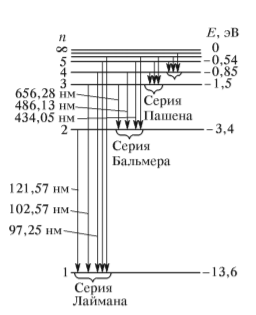
\includegraphics[height=6cm]{spv.png}
\end{center}
\ECaption{Уровни энергии атома водорода и образование спектральных линий.}
\end{wrapfigure}

Исходя из модели атома Бора электроны в атоме могут находиться на определенных энергетических уровнях, определяемых формулой:

\begin{equation}
E_n= -\frac{2\pi^2m_e e^4 Z^2}{h^2}\frac{1}{n^2}.
\end{equation}

Исходя из экспериментального спектра, показанного на рис.1, и формулы (2) видим, что линии спектра наблюдаются в виде серий с характерным $n$. В этой работе будет исследоваться серия Бальмера, для которой $n=2$. То, что наблюдается именно спектр серии Бальмера обеспечивает тот факт, что только эта серия находится в области видимого света, а установка предполагает наблюдение только видимого спектра. 

Величины $m$ для первых 4 линий серии $ H_{\alpha} $, $ H_{\beta} $, $ H_{\gamma} $, $ H_{\delta} $ равны соответственно 3, 4, 5 и 6.

Постоянная Ридберга определяется из соотношения для энергии основного состояния атома:
\begin{equation}
E = -\frac{m_ee^4}{2h^2}Z^2 = -RZ^2.
\end{equation}

\section*{Градуировка спектрометра}

\subsection*{Экспериментальная установка}

\begin{figure}[h]
\begin{center}
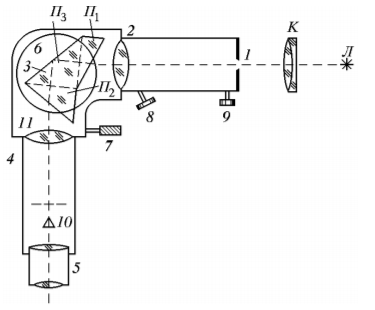
\includegraphics[width=0.7\textwidth]{ust}
\end{center}
\ECaption{Схема экспериментальной установки. С помощью линзы можно было фокусировать источник света в щели спектрометра, от чего зависела четкость наблюдаемых спектральных линий. С помощью барабана 7 ставилось соответствие между длиной волны линии и её положением. Эта зависимость не является линейной, поэтому необходима градуировка спектрометра.}
\end{figure}

\subsection*{Градуировка по неоновой и ртутной лампам}

Градуировка спектрометра производилась с помощью известных спектров: неоновой и ртутной ламп. С помощью таблиц цветов спектра, и так же их рисунков, можно было поставить соответствие между известной линией и ее положением на барабане. Результаты представлены на таблице 1.

\begin{table}[h]
\begin{center}
\begin{tabular}{|cc|c|cc}
\hline
\rowcolor[HTML]{9698ED} 
неон                                                                                \hspace{1 cm} &            \hspace{2 cm}                  & .                         & ртуть                                                                              \hspace{1 cm} & \multicolumn{1}{c|}{\cellcolor[HTML]{9698ED} }     \\ \hline
\multicolumn{1}{|c|}{$\varphi$, $^{\circ}$} & $\lambda$, $A$    & \cellcolor[HTML]{9698ED}. & \multicolumn{1}{c|}{$\varphi$, $^{\circ}$} & \multicolumn{1}{c|}{$\lambda$, $A$ }    \\ \hline
\rowcolor[HTML]{9698ED} 
\multicolumn{1}{|c|}{\cellcolor[HTML]{9698ED}1888}                                   & 5331                       & .                         & \multicolumn{1}{c|}{\cellcolor[HTML]{9698ED}2554}                                   & \multicolumn{1}{c|}{\cellcolor[HTML]{9698ED}6907} \\ \hline
\multicolumn{1}{|c|}{2148}                                                           & 5852                         & \cellcolor[HTML]{9698ED}. & \multicolumn{1}{c|}{2314}                                                           & \multicolumn{1}{c|}{6234}                         \\ \hline
\rowcolor[HTML]{9698ED} 
\multicolumn{1}{|c|}{\cellcolor[HTML]{9698ED}2160}                                   & 5882                         & .                         & \multicolumn{1}{c|}{\cellcolor[HTML]{9698ED}2116}                                   & \multicolumn{1}{c|}{\cellcolor[HTML]{9698ED}5791} \\ \hline
\multicolumn{1}{|c|}{2190}                                                           & 5945                         & \cellcolor[HTML]{9698ED}. & \multicolumn{1}{c|}{2100}                                                           & \multicolumn{1}{c|}{5770}                         \\ \hline
\rowcolor[HTML]{9698ED} 
\multicolumn{1}{|c|}{\cellcolor[HTML]{9698ED}2208}                                   & 5976                         & .                         & \multicolumn{1}{c|}{\cellcolor[HTML]{9698ED}1920}                                   & \multicolumn{1}{c|}{\cellcolor[HTML]{9698ED}5461} \\ \hline
\multicolumn{1}{|c|}{2234}                                                           & 6030                         & \cellcolor[HTML]{9698ED}. & \multicolumn{1}{c|}{1500}                                                           & \multicolumn{1}{c|}{4916}                         \\ \hline
\rowcolor[HTML]{9698ED} 
\multicolumn{1}{|c|}{\cellcolor[HTML]{9698ED}2256}                                   & 6074                         & .                         & \multicolumn{1}{c|}{\cellcolor[HTML]{9698ED}834}                                    & \multicolumn{1}{c|}{\cellcolor[HTML]{9698ED}4358} \\ \hline
\multicolumn{1}{|c|}{2264}                                                           & 6096                         & \cellcolor[HTML]{9698ED}. & \multicolumn{1}{c|}{346}                                                            & \multicolumn{1}{c|}{4047}                         \\ \hline
\multicolumn{1}{|c|}{\cellcolor[HTML]{9698ED}2284}                                   & \cellcolor[HTML]{9698ED}6143 & \cellcolor[HTML]{9698ED}. &                                                                                     &                                                   \\ \cline{1-3}
\multicolumn{1}{|c|}{2292}                                                           & 6164                         & \cellcolor[HTML]{9698ED}. &                                                                                     &                                                   \\ \cline{1-3}
\multicolumn{1}{|c|}{\cellcolor[HTML]{9698ED}2316}                                   & \cellcolor[HTML]{9698ED}6217 & \cellcolor[HTML]{9698ED}. &                                                                                     &                                                   \\ \cline{1-3}
\multicolumn{1}{|c|}{2336}                                                           & 6267                         & \cellcolor[HTML]{9698ED}. &                                                                                     &                                             \hspace{2 cm}      \\ \cline{1-3}
\multicolumn{1}{|c|}{\cellcolor[HTML]{9698ED}2352}                                   & \cellcolor[HTML]{9698ED}6305 & \cellcolor[HTML]{9698ED}. &                                                                                     &                                                   \\ \cline{1-3}
\multicolumn{1}{|c|}{2362}                                                           & 6334                         & \cellcolor[HTML]{9698ED}. &                                                                                     &                                                   \\ \cline{1-3}
\multicolumn{1}{|c|}{\cellcolor[HTML]{9698ED}2380}                                   & \cellcolor[HTML]{9698ED}6383 & \cellcolor[HTML]{9698ED}. &                                                                                     &                                                   \\ \cline{1-3}
\multicolumn{1}{|c|}{2390}                                                           & 6402                         & \cellcolor[HTML]{9698ED}. &                                                                                     &                                                   \\ \cline{1-3}
\multicolumn{1}{|c|}{\cellcolor[HTML]{9698ED}2426}                                   & \cellcolor[HTML]{9698ED}6507 & \cellcolor[HTML]{9698ED}. &                                                                                     &                                                   \\ \cline{1-3}
\end{tabular}
\ECaption{Градуировка спектрометра. Значения барабана определяются в градусах с погрешностью в $2^{\circ}$.}
\end{center}
\end{table}

По полученным данным можно построить градуировочный график, изображенный на рис (3).

\begin{figure}[h!]
\begin{center}
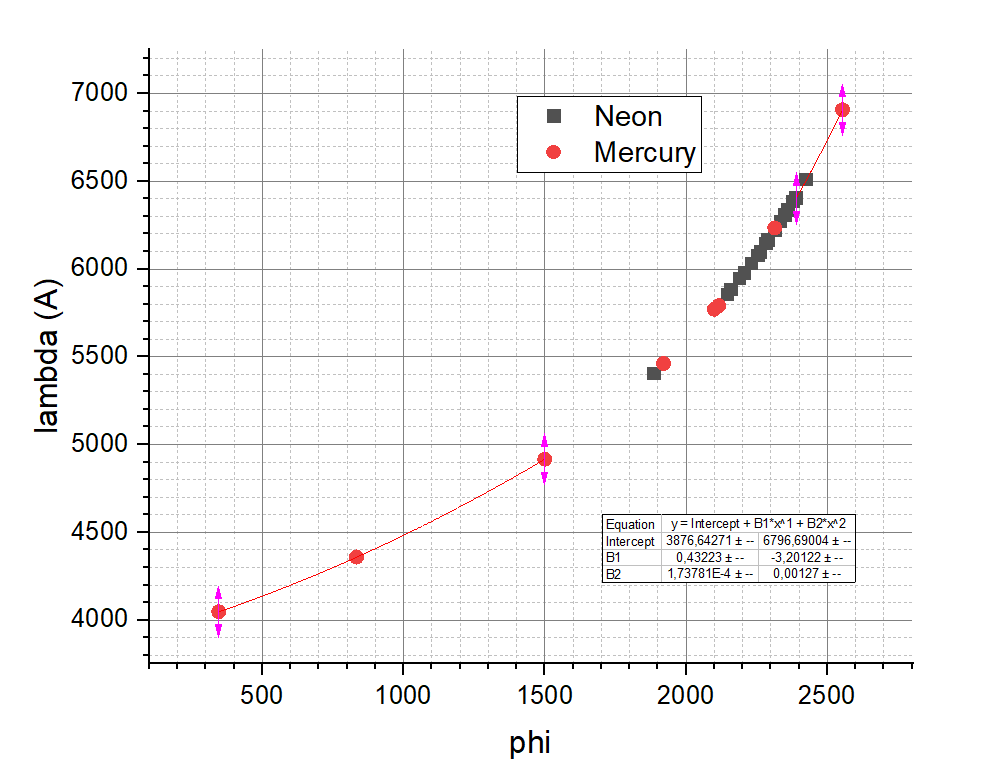
\includegraphics[width=0.9\textwidth]{gr1}
\end{center}
\ECaption{Градуировочная кривая по значениям спектра неона и ртутной лампы. Как видно, значения получены достаточно достоверно, что связано как с хорошей настройкой установки, так и методом измерения. В этой работе важным фактором является наличие параллакса между глазом, фиксирующей шкалой и линиями на экране. Чтобы его избежать, команда четко разделила обязанности, и градуировку снимал один человек (я) не меняя положения глаз, в то время как остальные фиксировали значения.}
\end{figure}

Как видно по графику, все точки хорошо аппроксимируются гладкой кривой. Так как функция этой кривой не может быть определена, то для градуировки лучше использовать метод частичной аппроксимации -- брать 3 ближайших точки от той, которую надо определить, и проводить по ним пораболу. Так как порабола по 3 точкам единственна, является гладкой кривой, то она может аппроксимировать значения с достаточно высокой точностью. Значения для линий водорода будут получены именно таким способом.

\newpage

\newpage
 
\section*{Спектр водорода}

Измерения спектра водорода проводились тем же методом. Все точки были сняты по кругу дважды, чтобы уменьшить влияние изменения положения глаза в процессе измерения. На таблице 2 сразу представлены и значения длин волн, посчитанных с помощью калибровочной кривой.

\begin{table}[h]
\begin{center}
\begin{tabular}{|c|c|c|}
\hline
\rowcolor[HTML]{9698ED} 
$\phi$, $^{\circ}$ & $\lambda$, $A$ & $\lambda_{\text{teor}}$, $A$ \\ \hline
2438               & 6541           & 6562.8                       \\ \hline
\rowcolor[HTML]{9698ED} 
1450               & 4869           & 4861.3                       \\ \hline
806                & 4338           & 4340.5                       \\ \hline
\rowcolor[HTML]{9698ED} 
364                & 4057           & 4101.7                       \\ \hline
\rowcolor[HTML]{DAE8FC} 
806                & 4338           & 4340.5                       \\ \hline
\rowcolor[HTML]{9698ED} 
1446               & 4865           & 4861.3                       \\ \hline
\rowcolor[HTML]{DAE8FC} 
2436               & 6535           & 6562.8                       \\ \hline
\rowcolor[HTML]{C0C0C0} 
394                & 4074           & 4101.7                       \\ \hline
\rowcolor[HTML]{C0C0C0} 
352                & 4050           & 4101.7                       \\ \hline
\end{tabular}
\ECaption{ Данные за первый круг - первые 4 строки, за второй - следующие 3 строки. Последние 2 строки - линия $H_{\delta}$, снятая после того, как я отошел от остановки, так что эти данные менее достоверные в условиях эксперимента.}
\end{center}
\end{table}

Как видно, данные измерений 2 кругов, не считая 4 линию, почти одинаковы, так что можно считать, что методика измерений дает единственный результат.
В качестве результатов взяты данные первого круга.

Для иллюстрации точности данных построен график на рис. 4., на который добавлены длины волн линий, известных теоретически. Линия $H_{\delta}$ Выбивается из калибровочной кривой больше других, что связано с ошибкой эксперимента. Если считать погрешность измерения метода как половину ширины линии, то общая погрешность измерения положения линии определяется как:
\[\Delta = \sqrt{\Delta_{\text{метода}}^2 + \Delta_{\text{ц.д.}}^2 } \simeq 4^{\circ} \text{ (В случае всех измерений кроме } H_{\delta}).\] 
Измерения проводились при неизменной ширине линий, однако для наблюдения $H_{\delta}$ необходимо было увеличить ширину линии в 5 раз, из-за чего погрешность стала равной $15^{\circ}$. 

\begin{figure}[h!]
\begin{center}
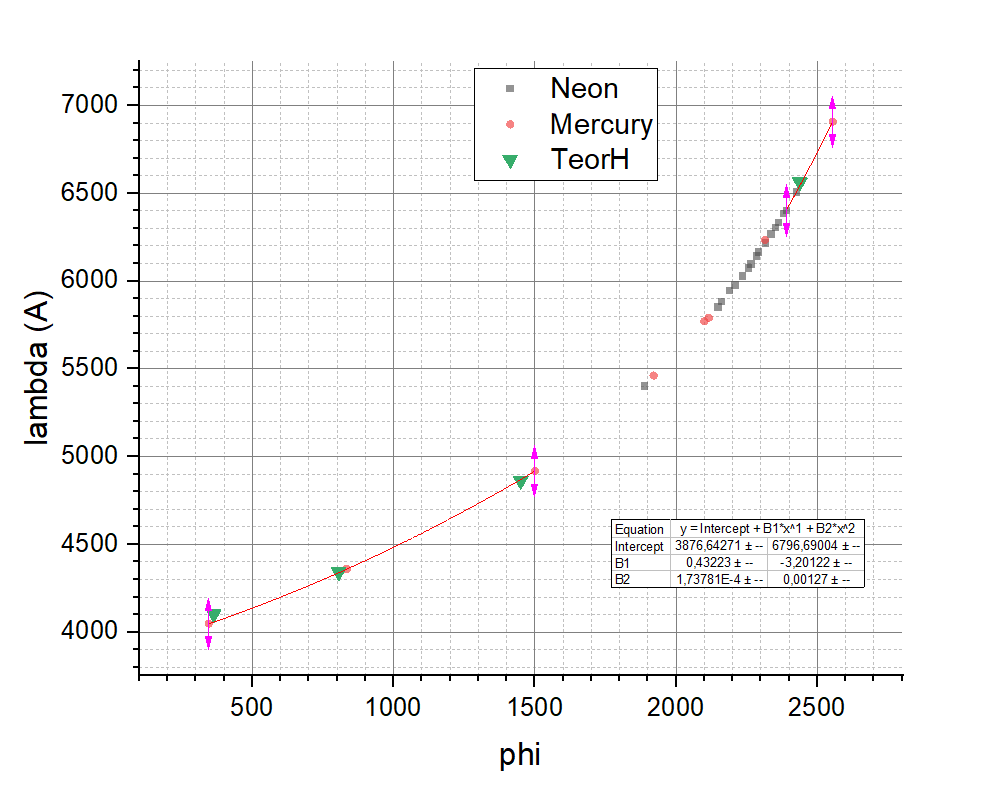
\includegraphics[width=0.9\textwidth]{gr2}
\end{center}
\ECaption{На графике контрастным точкам соответствуют теоретические значения длин волн линий и измеренными положениями линий на спектрометре. Как видно, теоретические данные близки к данным, полученным с калибровочной кривой.}
\end{figure}

\subsection*{Постоянная Ридберга}

Из формулы (1) для спектра водорода получаем 
\[\dfrac{1}{\lambda_m} = R\left( \frac{1}{4} - \frac{1}{m^2}\right) .\]
Тогда по этой зависимости можно построить линеаризованный график, изображенный на рис. 5.

\begin{figure}[h!]
\begin{center}
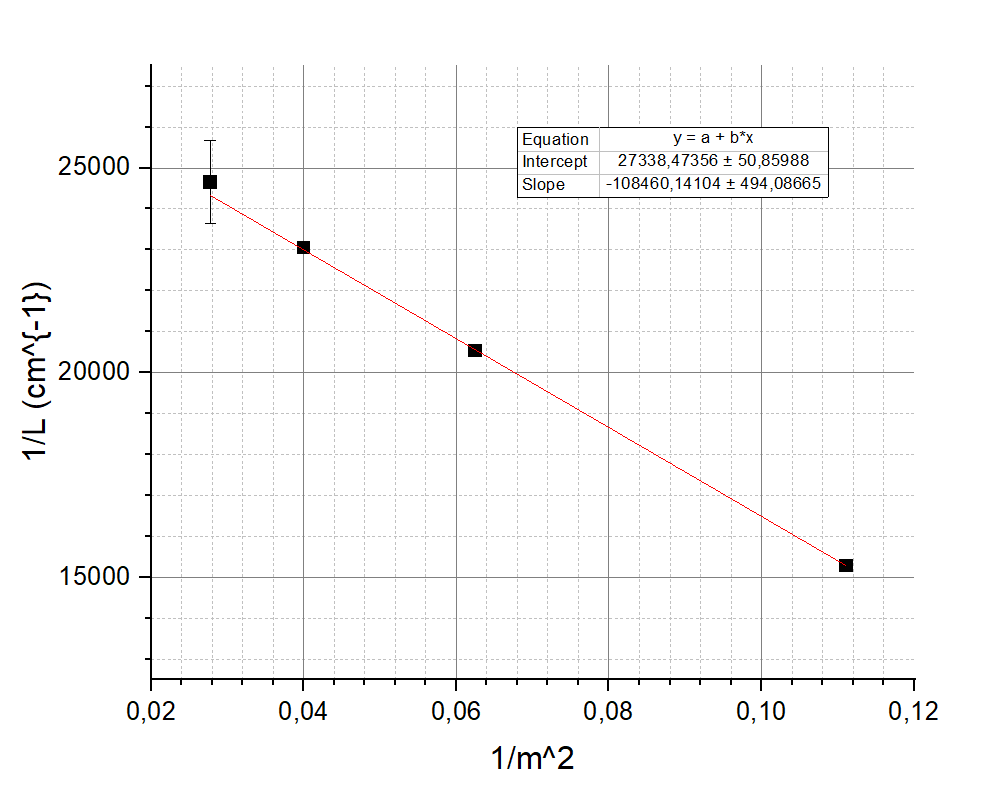
\includegraphics[width=0.9\textwidth]{gr3}
\end{center}
\ECaption{График зависимости $\frac{1}{\lambda}(\frac{1}{m^2})$. Здесь заметно, что точка $H_{\delta}$ посчитана с намного более плохой точностью, чем остальные, однако все равно близка к аппроксимирующей прямой. }
\end{figure}

Полученное значение постоянной Ридберга:
\[R = 108460 \pm 490 \text{ см}^{-1},\]
что вполне соответствует теоретическому значению:
\[R_{\text{teor}} = 109677,6 \text{ см}^{-1}. \]

Исходя из (1) можем так же проверить сериальную закономерность:
\[n = \sqrt{\frac{-Slope}{Intercept}} = 1.99,\]
что должно равняться 2, и, в принципе, равняется. Так что можно утверждать, что производились измерения одной серии.

\section*{Вывод}

В процессе работы команда познакомилась с принципом работы спектрометра, определив способы наиболее точной градуировки и снятия данных. Было доказано, что в снятые точки принадлежат серии Бальмера, а полученное значение для постоянной Ридберга совпадает с теоретическим в 3 знаке, что свидетельствует о высокой точности эксперимента. Так же наблюдались все 4 спектральные линии серии, что является следствием хорошей настройки спектрометра. 







\end{document}